%!TEX root = ../documentation.tex
\chapter{Datenanalyse}
\label{ch:data_analysis}

\section{Bilddaten}
\newlength{\imagewidth}

Wir betrachten zunächst die Bilddaten aus dem Datensatz und stellen anhand von geeigneten Beispielen und Analysen heterogene Eigenschaften dieser dar, welche sich für das Training unserer Modelle als problematisch erweisen könnten.

\begin{figure}[ht]
	\centering
	\begin{subfigure}[b]{0.45\textwidth}
		\includegraphics[width=\textwidth]{../images/34308.jpeg}
		\caption{34308.jpeg\\Originalgröße 1524 x 1516 Pixel}
	\end{subfigure} \hfill
	\begin{subfigure}[b]{0.45\textwidth}
		\includegraphics[width=\textwidth]{../images/65415.jpg}
		\caption{65415.jpg\\Originalgröße 369 x 320 Pixel}
	\end{subfigure}
	\caption{Zwei Bilder männlicher Patienten aus dem Datensatz}
\end{figure}

Die Beispiele (a) und (b) lassen einen deutlich unterschiedlichen Kontrast erkennen. Bei Beispiel (a) handelt es sich zudem um ein Farbbild während es sich bei Beispiel (b) um ein Schwarzweißbild handelt. Die beiden Bilder weisen unterschiedliche Dimensionen auf.\\
Diese heterogenen Eigenschaften zeigen Komplexität innerhalb des Datensatzes, welche von einem gelernten Model entsprechend wiedergespiegelt werden müsste. Es ist also angebracht die Daten mittels geeigneter Vorverarbeitung zu homogenisieren.

\pagebreak

Insgesamt werden die Unterschiede in Dimension und Farbe von den folgenden Grafiken dargestellt.

\begin{figure}[H]
	\centering
	\settowidth{\imagewidth}{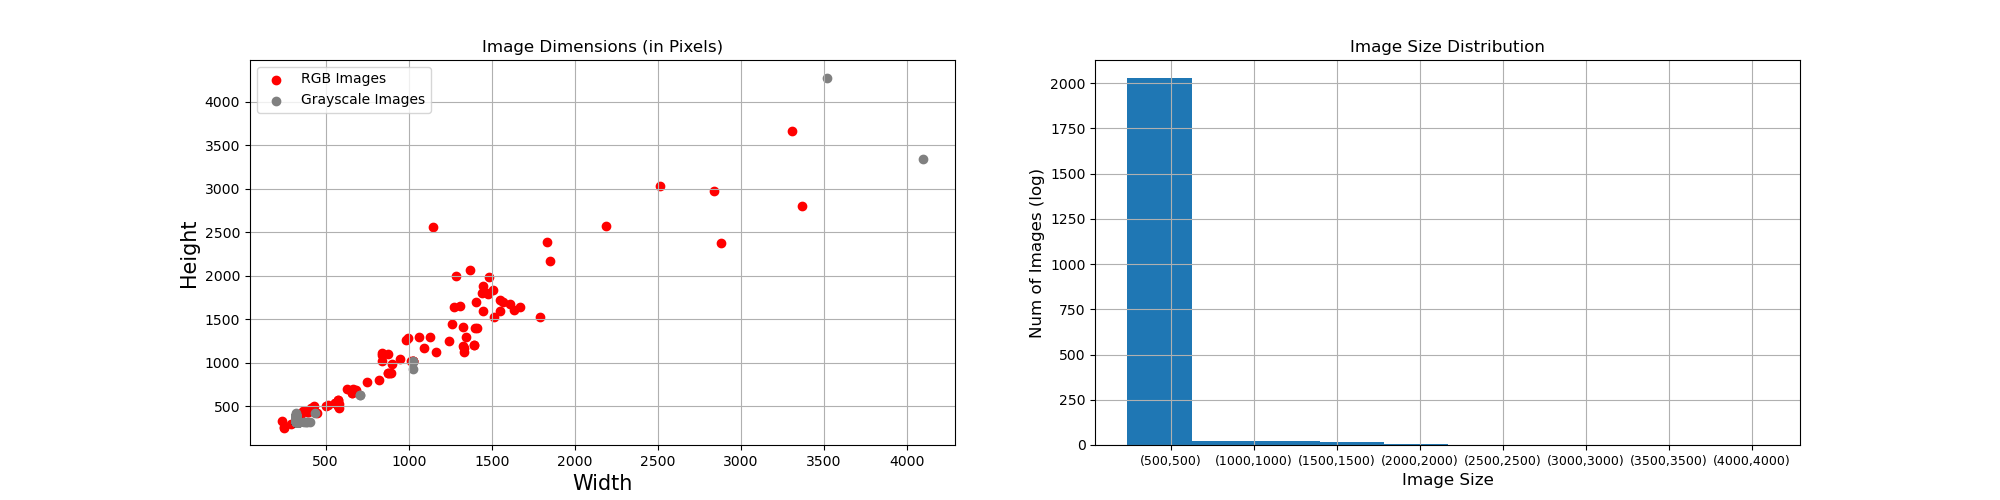
\includegraphics{../results/image_sizes.png}}
	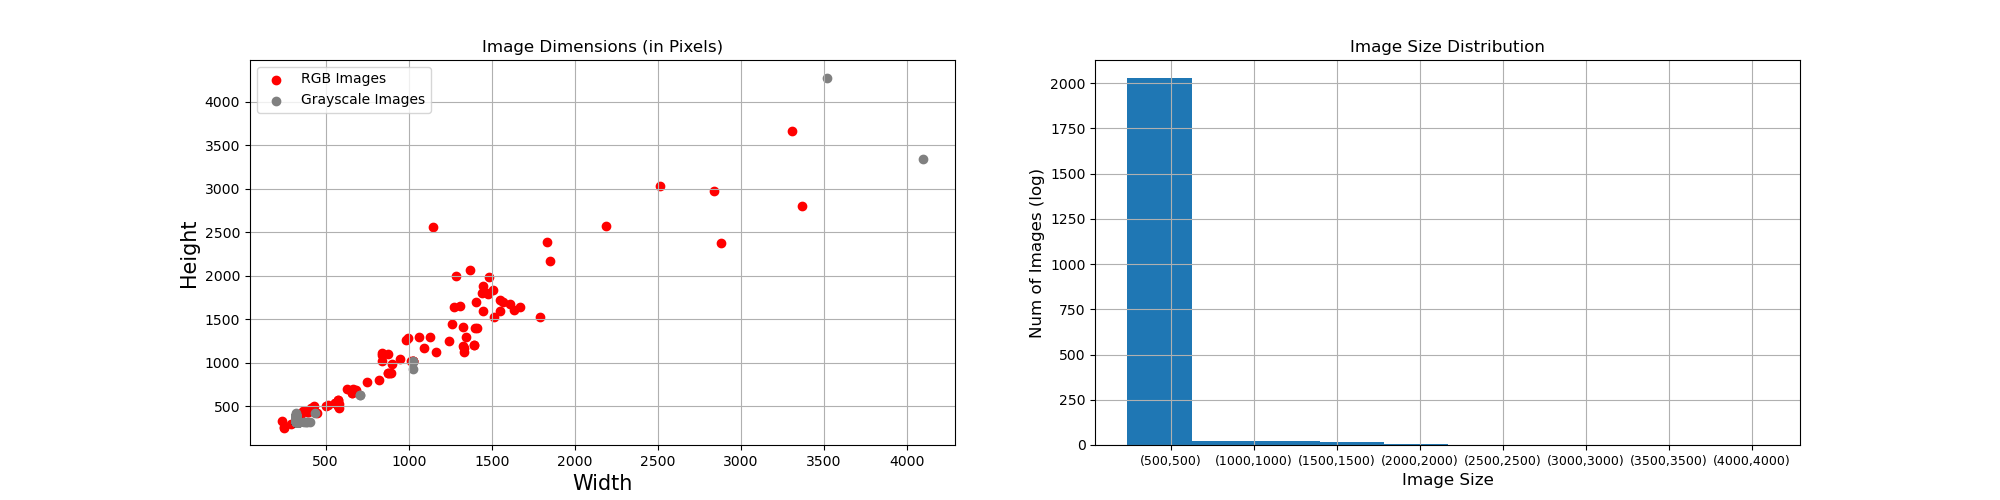
\includegraphics[trim=110px 0 0.5\imagewidth{} 0, clip,width=0.9\textwidth]{../results/image_sizes.png}
	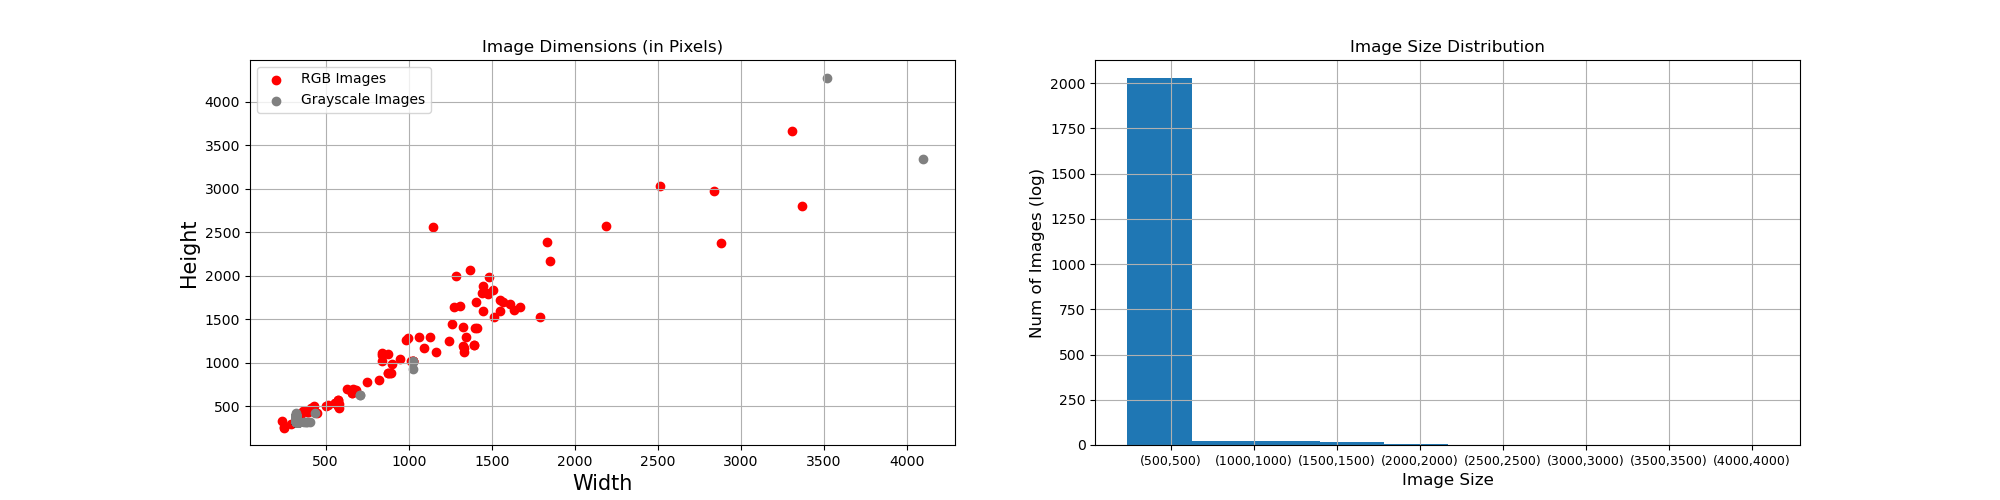
\includegraphics[trim=0.5\imagewidth{} 0 110px 0, clip,width=0.9\textwidth]{../results/image_sizes.png}
	\caption{Verteilung der Bilddimensionen}
\end{figure}

Von den 2100 Bildern des Datensatzes sind 92 Farbbilder und 2008 Schwarzweißbilder. Ein Großteil der Dimensionen ist im Bereich von 320 x 320 Pixeln angeordnet.

\section{Klassen}

Wir betrachten nun die Verteilung der Klassen über den Datensatz in zwei Konstellationen. In der ersten Konstellation wird jede Krankheit von einer eigenen Klasse repräsentiert, während in der zweiten Konstellation alle Krankheiten mit Ausnahme von COVID-19 zu einer Klasse zusammengefasst werden.

\begin{figure}[H]
	\centering
	\settowidth{\imagewidth}{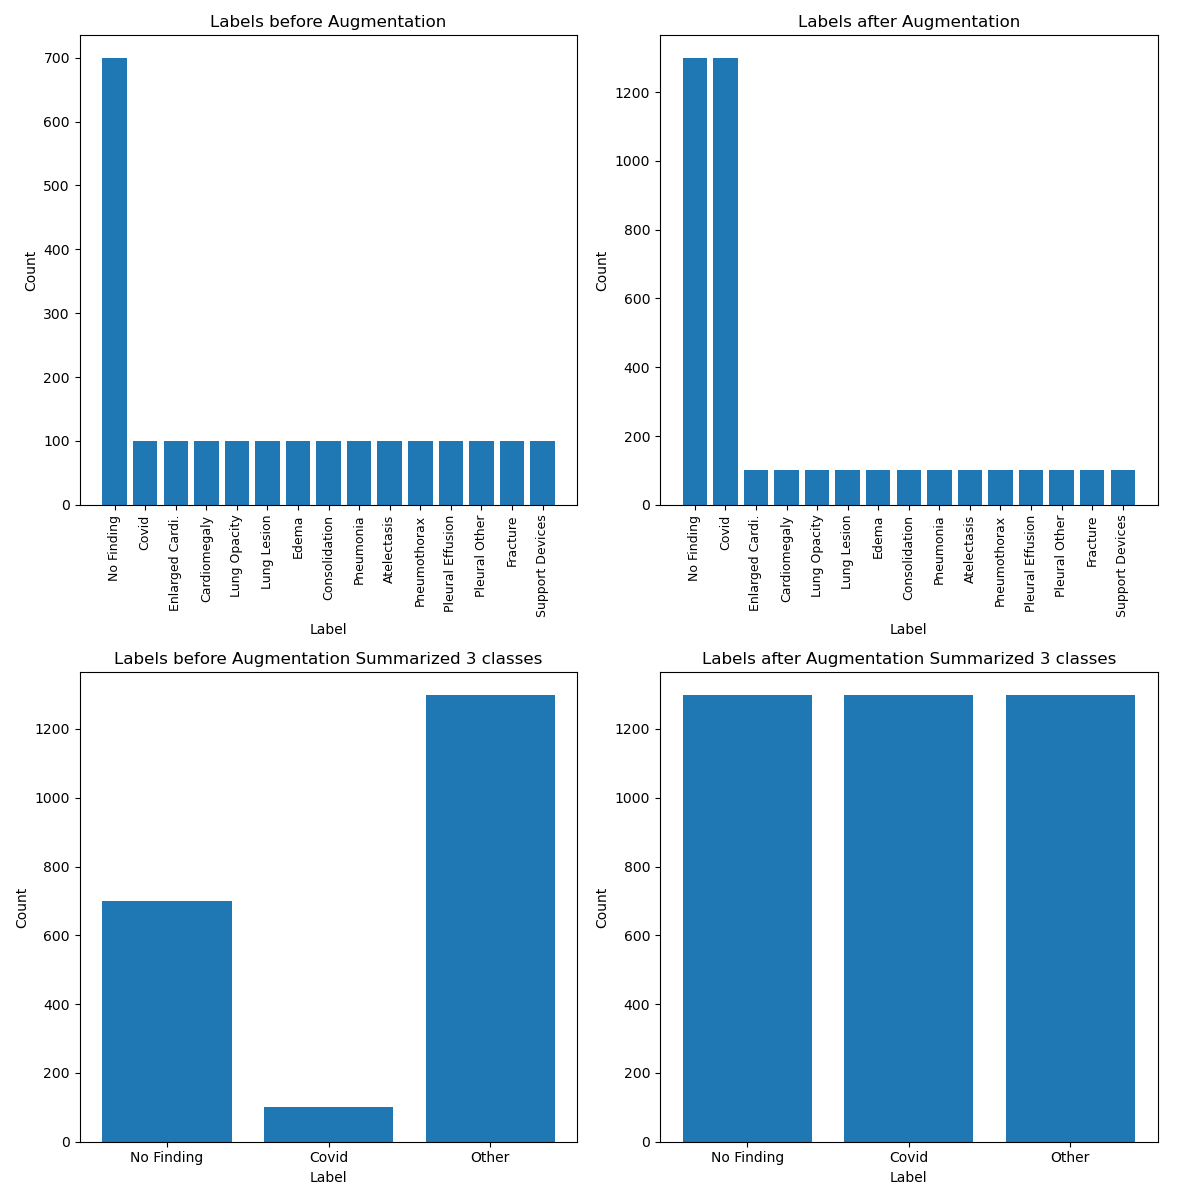
\includegraphics{../results/balancing.png}}
	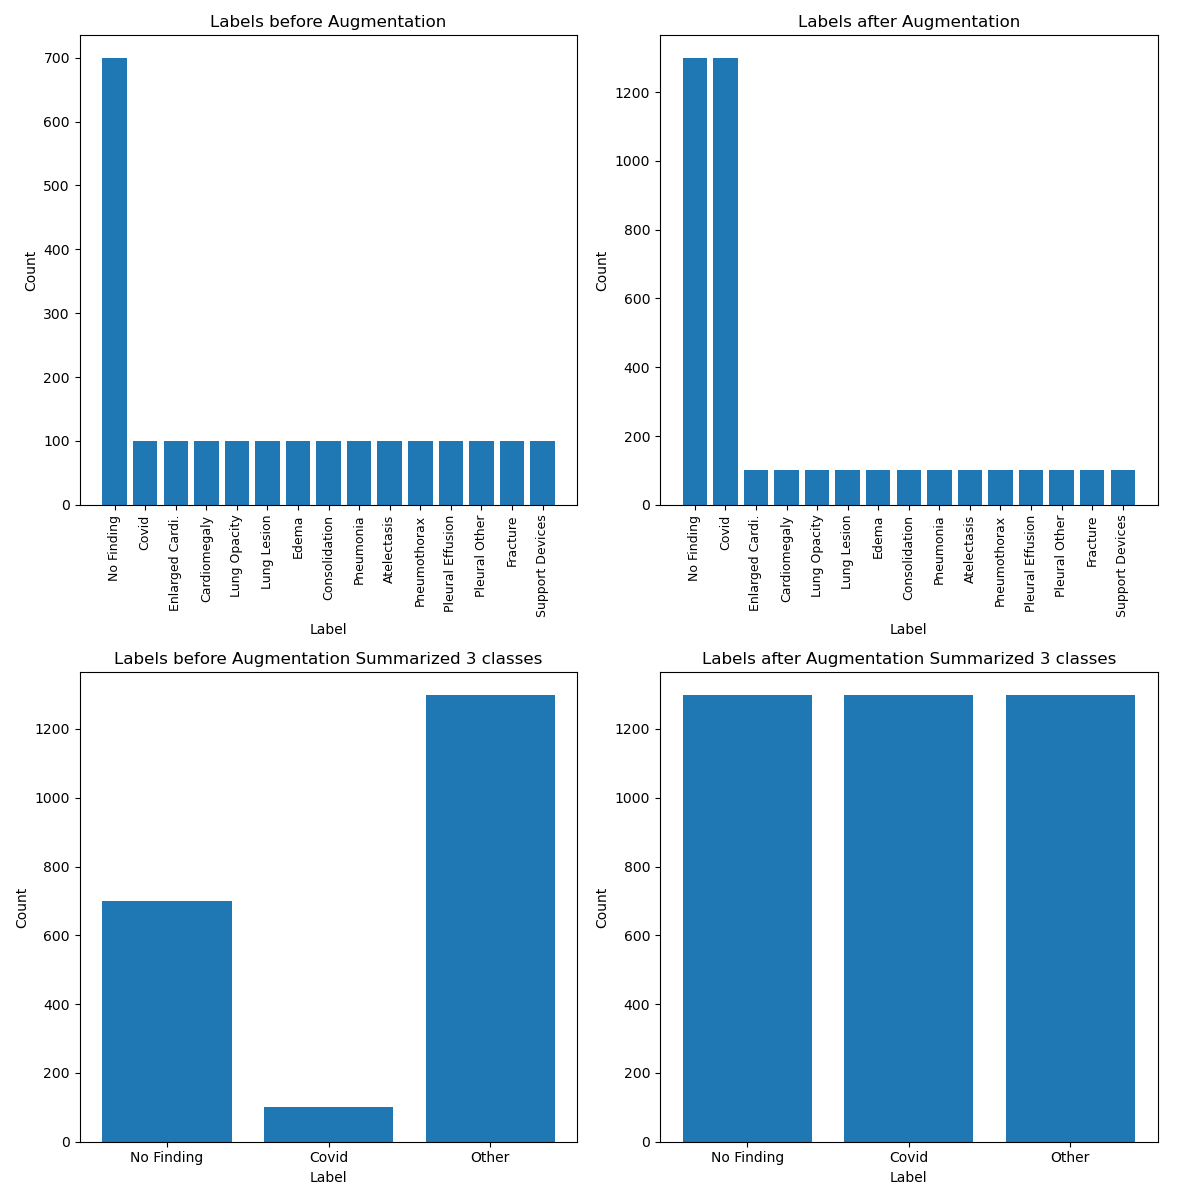
\includegraphics[trim=0 0 0.51\imagewidth{} 0, clip,width=0.275\imagewidth{}]{../results/balancing.png}
	\caption{Verteilung der Klassen}
\end{figure}

In der ersten Konstellation sind die Krankheiten gleichverteilt. Pro Krankheit existieren 100 Beispielbilder. Insgesamt existieren 1400 Bilder für die Krankheitsklassen und 700 ohne Befund.\\
In der zweiten Konstellation ist der Anteil an COVID-19 Erkrankungen im Vergleich zu den anderen Klassen relativ gering.
Um eine gute Generalisierungsfähigkeit sicherzustellen, ist es hier sinnvoll zusätzliche Trainingsbeispiele aus der COVID-19 Klasse bereitzustellen.

Wir betrachten ebenfalls die Verteilung der Features Alter und Geschlecht innerhalb der Klasse der COVID-19 Erkrankungen.

\begin{figure}[ht]
	\centering
	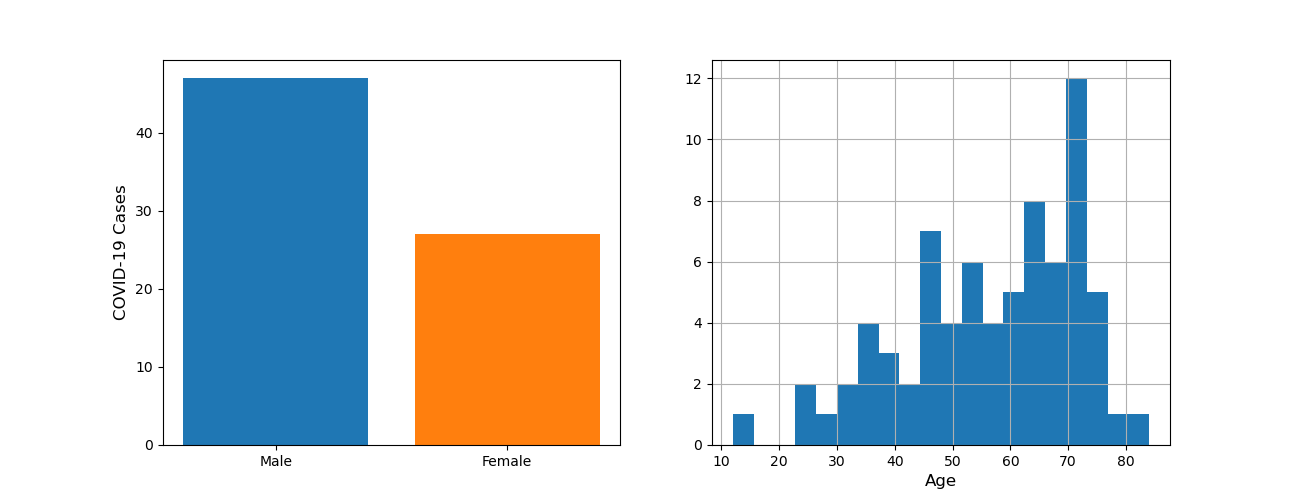
\includegraphics[width=\textwidth]{../results/features_analysis.png}
	\caption{Analyse der Features Alter und Geschlecht bei COVID-19 erkrankten Patienten}
\end{figure}

Die Anteile von männlichen Patienten ist höher als der von weiblichen. Ebenfalls sind Daten von eher älteren Patienten vorhanden. Das Durchschnittsalter beträgt 56,46 Jahre.\\
Eventuell sind zusätzliche Maßnahmen zur Entzerrung der Daten sinnvoll.

\section{Implementierung}

Für die Datenanalyse steht das Python-Script \verb|data_analysis.py| zur Verfügung.

Dieses kann folgendermaßen aufgerufen werden:

\begin{verbatim}
python preprocessing/data_analysis.py [-h] [dataset] [output]
\end{verbatim}

Die positionalen Argumente \verb|dataset| und \verb|output| geben jeweils den Pfad zum Datensatz- und zum Ausgabeverzeichnis an.
Über den optionalen Parameter \verb|-h| bzw. \verb|--help| kann eine Programmhilfe ausgegeben werden.